\documentclass[technicalreport]{ieicej}
\usepackage[dvipdfmx]{graphicx}
\usepackage[T1]{fontenc}
\usepackage{lmodern}
\usepackage{textcomp}
\usepackage{latexsym}
\usepackage{amsmath}
\usepackage{cite}
\usepackage{tikz}
\usepackage{geometry}
\usepackage{url}
\usepackage{schemabloc}
\usepackage{tikz}
\usepackage{makecell}
\usetikzlibrary{arrows}

\usetikzlibrary{positioning,fit,calc}
\tikzset{block/.style={draw, thick, text width=1cm, minimum height=0.5cm, align=center}, line/.style={-latex}}  

\renewcommand{\figurename}{Fig.} % name the picture Fig.num
\renewcommand{\tablename}{Table } % name the table Table num
\renewcommand{\refname}{REFERENCE} % insert reference 

%调整文件显示位置和纸张
\geometry{
	a4paper,
	total={170mm,257mm},
	left=20mm,
	top=20mm,
}

\hoffset=-5mm
\voffset=-5mm

\def\IEICEJcls{\texttt{ieicej.cls}}
\def\IEICEJver{3.0}
\newcommand{\AmSLaTeX}{%
$\mathcal A$\lower.4ex\hbox{$\!\mathcal M\!$}$\mathcal S$-\LaTeX}
\def\BibTeX{{\rmfamily B\kern-.05em{\scshape i\kern-.025em b}\kern-.08em
T\kern-.1667em\lower.7ex\hbox{E}\kern-.125em X}}

\jtitle{M1課題レポート 第2回}
\jsubtitle{}
\etitle{Technical Report for M1 Labwork 2nd}
\esubtitle{}
\authorlist{
\authorentry[liuyuchen@radio.ict.e.titech.ac.jp]{劉 ゆ辰}{Yuchen Liu}{Titech}
}

\affiliate[Titech]{東京工業大学 〒152-8550 東京都目黒区大岡山2-12-1}
{Tokyo Institute of Technology,~~2-12-1, O-okayama, Meguro-ku, Tokyo, 152-8550 Japan}

\begin{document}

\begin{eabstract}
In this second C workshop, we use C language to simulate workflow of DQPSK modulation and non-coherent demodulation system over AWGN channel with phase shift. We first introduce the backgroud knowledege of DQPSK modulation and non-coherent demodulation. Next, we state the whole system desgin and simulation condition. From the result, we can see non-coherent demodulation achieve acceptable performance over phase shift channel.
\end{eabstract}

\maketitle

\section{Introduction}
In this Labwork, we introduce phase shift over AWGN channel, which will make coherent reception become unachievable. Phase shift is very common in wireless communication. To handle this phenomenon, we deploy diffential coding at transimtter and non-coherent reception.\par
At transmitter, Differential Quadrature Reference Phase Shift Keying (DQPSK) is adpoted. Compare to general Quadrature Reference Phase Shift Keying (QPSK), bit signal is not correspond to modulation symbol, but correspond to the differential between two symbols.The current phase of carrier is the summation of previous phase and the differential. The mapping of bit signal and differential phase is shown in Table 1.\par
At receiver, non-coherent reception counteract the effect of phase shifting by demodulate signal by the multiplication of previous symbol and current symbol. The mathematics formula is shown as follow:
\begin{equation}
\begin{aligned}
d(i)&=r(i)\cdot r^*(i-1)\\
&=s(i)s^*(i)\\
&+\underbrace{s(i)n^*(i-1)e^{j\phi}+s^*(i-1)n(i)e^{-j\phi}+n(i)n^*(i-1)}_{\rm redundant\quad part}
\end{aligned}
\end{equation}
In (1) we can see after multiplication, the majority value of equation is $s(i)s^*(i-1)$ which is equal to the value of differential symbol, which we can see from:
\begin{equation}
\begin{aligned}
s(i)s^*(i-1)&=e^{j\delta\theta_i}s(i-1)s^*(i-1)\\
&=e^{j\delta\theta_i}|s(i-1)|^2\\
&=e^{j\delta\theta_i}\\
&=d(i)
\end{aligned}
\end{equation}
Thus, we can demodulate signal from non-coherent reception over channel with phase shift and redundant part can be seen as noise. Because the redundant part is larger than $n(i)$, thus the performance of non-coherent reception will be worse than coherent reception when there isn't any phase shift.

\begin{table}[tbp]
	\begin{center}
	\caption{MAPPING TABLE OF PHASE}
	\begin{tabular}{lll}
	\hline
	\textbf{bitA} & \textbf{bitB} & \textbf{$\Delta\theta_{i}$} \\
	\hline
	\makecell[c]{0} & \makecell[c]{0} & \makecell[c]{$0$} \\
	\makecell[c]{1} & \makecell[c]{0} & \makecell[c]{$\frac{pi}{2}$} \\
	\makecell[c]{1} & \makecell[c]{1} & \makecell[c]{$\pi$} \\
	\makecell[c]{1} & \makecell[c]{0} & \makecell[c]{$\frac{3\pi}{2}$} \\
	\hline
	\end{tabular}
	\end{center}
\end{table}

\begin{figure}[ht]
	\begin{center}
		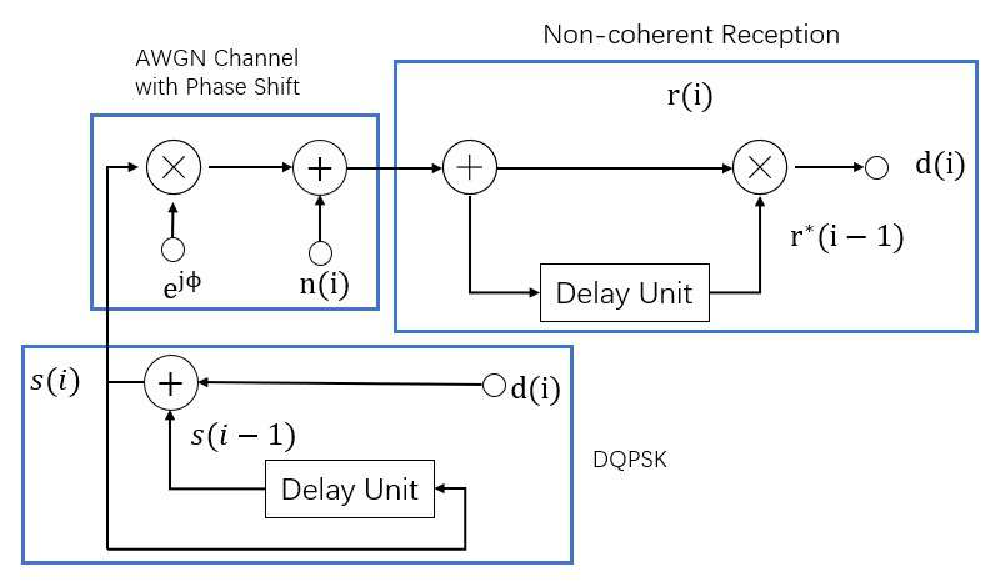
\includegraphics[scale=0.5]{fig/system.pdf}
		\caption{System Block Diagram}
		\label{fig:label}
	\end{center}
\end{figure}

\section{Simulation Desgin}
Fig.1 shows the whole system architecture, the phase shift is realized by multiply a rand varible $\phi$ obey uniform distribution to signal $s(i)$. The channel formula is shown as follow:
\begin{equation}
r(i)=s(i)e^{j\phi}+n(i)
\end{equation}
And theortical BER for DQPSK over phase shift AWGN channel can be shown as follow:
\begin{equation}
P_e \simeq \frac{1}{2}{\rm erfc}\left \{ 2\sqrt{\gamma}\sin(\frac{\pi}{8}) \right \}
\end{equation}
The erfc function is ${\rm erfc}=\frac{2}{\sqrt{\pi}}\int_{x}^{+\infty}e^{-\eta^2}d\eta$. And $\gamma$ in the equation repersents $E_b/N_0$ which is not in dB.\par
Simulation condition can be shown in Table 2.

\begin{table}[hb]
	\begin{center}
	\caption{SIMULATION CONDITIONS}
	\label{tbl:simu}
	\small
	\begin{tabular}{ll}
	\hline
	ITEMS & CONDITIONS\\
	\hline
	Moduation Method & DQPSK \\
	Transmission Bits & 128 \\
	Channel & AWGN with Phase Shift \\
	Detection & Noncoherent/Coherent Detection \\
	Number of Trials & $10^{6}$\\
	Distribution of Phase Shift & ${\rm U}[0,2\pi]$\\
	\hline
	\end{tabular}
	\end{center}
\end{table}

\section{Simulation Result and Conclusion}
We can see the simulation result from Fig.2 and Fig.3. Fig.2 shows the Bit Error Rate (BER) over AWGN channel without phase shift when the SNR starts from 0 dB to 11 dB, which we can see the non-coherent reception perform worse in BER under such situation. While in the Fig.3, BER of coherent reception over AWGN with phase shift is completely inacceptable, but the coherent reception have same performance as when there is no phase shift.
In conclusion, non-coherent reception provide acceptable BER performance over phase shift AWGN channel, although the peformance is worse than coherent reception when there isn't any phase shift. On the other hand, non-coherent doesn't need knowlege of carrier, which is another advantage over coherent reception.

\begin{figure}[tbp]
	\begin{center}
		\vspace{0cm}
		\includegraphics[width=\linewidth,clip]{fig/without_shift.eps}
		\caption{Coherent Reception and Non-coherent Reception Without Phase Shift}
		\label{fig:sample}
	\end{center}
\end{figure}

\begin{figure}[tbp]
	\begin{center}
		\vspace{0cm}
		\includegraphics[width=\linewidth,clip]{fig/phase_shift.eps}
		\caption{Coherent Reception and Non-coherent Reception With Phase Shift}
		\label{fig:sample}
	\end{center}
\end{figure}

\end{document} 